% -*-mode: Latex-*-
% !TEX root = thesis.tex
% paper: ...
% authors: simon maurer
%
% file: rts.tex
% contents: runtime systems, experimentation, toolchain
% Sccs-Id: %W% %G%
\chapter{Toolchain for Streamix}
\label{chap_tool}

In this chapter I will give some technical details about the implementation of the compiler of the coordination language \gls*{smx}, the permanent blocking analysis, a runtime system for \gls*{smx} programs, and a preprocessor for the runtime system.
In order to build an application, with \glspl*{ccomp} being written in C/C++ and the coordination aspects being described by \gls*{smx}, the \gls*{smx} toolchain is used as described in the following list.
\begin{enumerate}
    \item The \gls*{smx} compiler \texttt{smxc} takes a \gls*{smx} file as input and produces a network dependency graph, annotated with network information such as whether inputs and outputs are decoupled, clock rates, and whether boxes are pure and/or static.
        Further, for each user-defined \gls*{ccomp} a graph file is produced, describing the \gls{sia} of the \gls*{ccomp}.
        Optionally, the compiler takes user-defined \gls{sia} descriptions of \glspl*{ccomp} as an input if the interaction protocol of the \gls*{ccomp} does not follow a default behaviour.
    \item The \gls{rts} preprocessor \texttt{smxrtsp} takes the network dependency graph, generated by the \gls*{smx} compiler, as an input and generates compilable C code, using function calls and macros defined in the \gls*{smx} runtime system library.
        Additionally, the \gls{rts} preprocessor generates the dependency graph of the \gls{pnsc} where only synchronous channels are used and \gls{fifo} channels are represented as processes.
        It further produces \gls{sia} description files for implicitly generated \gls{pnsc} processes such as channels and routing nodes.
    \item The permanent blocking analysis \texttt{smxsia} takes the \gls{pnsc} dependency graph and the interface descriptions of all processes as input (this includes automatically generated \gls{sia} files by the compiler and the runtime system preprocessor as well as the user-defined \glspl{sia} passed to the \gls*{smx} compiler) and checks the network for potential permanent blocking situations.
    \item Finally, the executable application code is created by compiling the \gls*{ccomp} implementations, the generated files by the runtime system preprocessor, and by linking the runtime system library and the libraries used by the \gls{rts}.
\end{enumerate}

\Fig{\ref{fig_toolchain}} provides a schematic overview of the build process described above.
The white boxes represent the executables described above and the unframed elements represent inputs and outputs.
The inputs in the grey area represent the inputs provided by the user.
%------------------------------------------------------------------
\begin{figure}[bht]
    \TopFigSpace
    \centering
    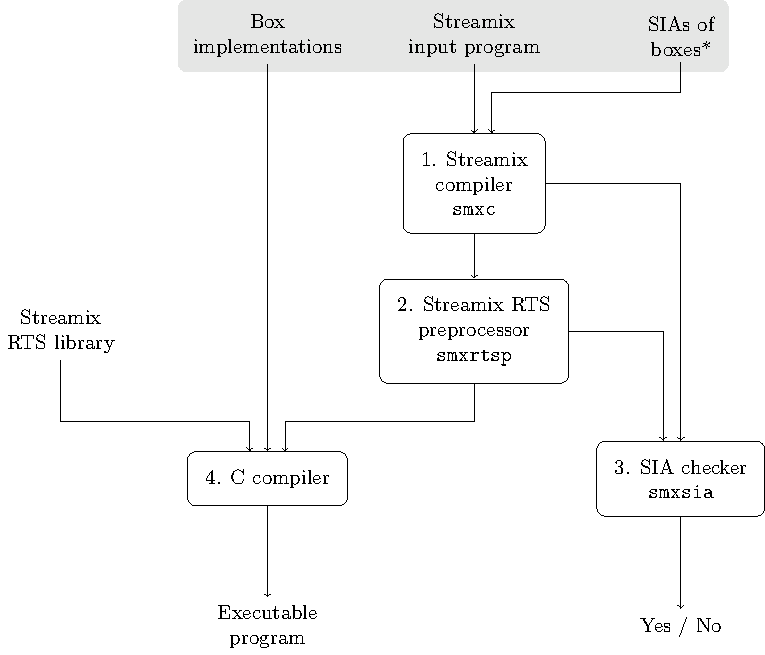
\includegraphics[width=12cm]{fig/toolchain.pdf}
    \CaptionFigSpace
    \caption{A schematic overview of the toolchain for \gls*{smx}.}
    \label{fig_toolchain}
    \BotFigSpace
\end{figure}
%------------------------------------------------------------------

I provide a root project with a link to all tools and some examples as a git repository on GitHub.
The source code for each tool is provided as a separate git repository where the code is commented respecting the \emph{Doxygen}\footnote{The homepage of the \emph{Doxygen} project: \url{http://www.stack.nl/~dimitri/doxygen/}} syntax.
For each repository the API documentation can be generated with the command \texttt{make doc}.
Here are the links to the different repositories:
\begin{description}
    \item[Root Project:] \url{https://github.com/moiri/streamix}
    \item[The RTS Library:] \url{https://github.com/moiri/streamix-rts}
    \item[\texttt{smxc} - The Compiler:] \url{https://github.com/moiri/streamix-c}
    \item[\texttt{smxrtsp} - The RTS Preprocessor:] \hfill \\
        \url{https://github.com/moiri/streamix-graph2c}
    \item[\texttt{smxsia} - The Permanent Blocking Analysis:] \hfill \\
        \url{https://github.com/moiri/streamix-sia}
\end{description}

The following list provides a brief overview of the examples that are available on GitHub.
I kept the examples simple to perform isolated tests with the network operators provided by \gls*{smx}.
All examples can easily be adapted, \eg~decoupling of ports, adding rate bounds or temporal firewalls, due to the exogenous nature of \gls*{smx}.
Each example can be compiled with the command \texttt{make}.
The command \texttt{make run} executes the compiled example and the command \texttt{make valgrind} uses \emph{Valgrind}\footnote{The project homepage of \emph{valgrind} can be found here: \url{http://valgrind.org/}} to execute and analyse the compiled example.

\begin{description}
    \item[\texttt{class.smx}] performs a serial composition of four nets where two nets refer to the same box declaration.
        This example serves to show the capability of \gls*{smx} to instantiate the same box declaration multiple times and allowing to concatenate the nets due to port collections.
    \item[\texttt{copy.smx}] demonstrates the implicit creation of a diverging routing node due to a parallel composition of two nets with the same input name.
    \item[\texttt{dboth.smx}] serves to demonstrate the communication over a \gls{fifo} channel that is decoupled on its input and output.
    \item[\texttt{din.smx}] serves to demonstrate the communication over a \gls{fifo} channel that is decoupled on its input.
    \item[\texttt{dout.smx}] serves to demonstrate the communication over a \gls{fifo} channel that is decoupled on its output.
    \item[\texttt{merge.smx}] demonstrates the implicit creation of a summing routing node due to a parallel composition of two nets with the same output name.
        Note that the non-deterministic parallel composition operator must be used here.
    \item[\texttt{simple.smx}] performs a serial composition between two nets and demonstrates port renaming capabilities of \gls*{smx}.
    \item[\texttt{stream.smx}] performs a serial composition between two nets and demonstrates how to specify a buffer length in \gls*{smx}.
        The example requires inputs by the user over the standard input stream.
        The program terminates once the character \texttt{ESC} is received by the consumer.
    \item[\texttt{tb.smx}] demonstrates a rate-bound communication over a decoupled channel.
    \item[\texttt{tcp.smx}] serves as a simple example to show the support of \gls*{smx} for complex components.
        Note that in this example the port order of the box declarations does not correspond to the communication protocol of the interacting processes.
        In order to prevent an error message from the permanent blocking analysis tool \texttt{smxsia} a custom \gls{sia} description is provided in the file \texttt{tcp.sia}.
        I did this intentionally to provide an example where a custom \gls{sia} description is required.
    \item[\texttt{tt.smx}] demonstrates the support of \gls*{smx} for temporal firewalls and the time-triggered communication scheme.
\end{description}

This chapter is structured as follows:
First, in \Sect{\ref{sect_tool_rts}} I describe the \gls{rts} library of \gls*{smx} to give the reader an understanding of how a \gls*{smx} program is mapped onto a software architecture and then run on a hardware platform.
\Sect{\ref{sect_tool_smxc}} gives technical insight on the compiler of the coordination language \gls*{smx}.
In \Sect{\ref{sect_tool_smxrtsp}} I describe the \gls{rts} preprocessor and in \Sect{\ref{sect_tool_smxsia}} I provide an overview of the implementation of the permanent blocking analysis.
Finally, in \Sect{\ref{sect_tool_discussion}} I discuss the result and the limitations of the implementation and in \Sect{\ref{sect_tool_summary}} I summarise the chapter.

%==============================================================================
\section{The Streamix RTS Library}
\label{sect_tool_rts}
The \gls{rts} of \gls*{smx} defines the execution model of a \gls*{smx} program.
It maps \gls*{smx} language elements to run-time constructs that can be executed on a hardware platform.
The \gls*{smx} \gls{rts} library provides a set of functions and macros that allows to create, initialise, execute, and destroy such run-time constructs.

In the following I describe a prototype of an \gls{rts} library for \gls*{smx} which I implemented as a proof of concept for the \gls*{smx} language.
The \gls{rts} is implemented in C and targets x86 architectures running a Linux operating system.
The \gls{rts} library uses POSIX threads~\cite{posix2009} and the \emph{zlog}\footnote{The homepage of the \emph{zlog} project: \url{https://github.com/HardySimpson/zlog}} library.
Timers which I use for the rate-control mechanism, are created with the \emph{timerfd} API which limits the \gls{rts} to Linux systems with kernel version~2.6.25 and newer.

A \gls*{smx} program defines, simply put, a network of \glspl*{ccomp} which interact with each other via channels.
In the \gls{rts} each \gls*{ccomp} is represented as a POSIX thread and each channel is a static structure with mutex variables that allow to model the blocking behaviour of \gls{fifo} channels.
The \gls{rts} provides function macros to connect threads by channels according to the \gls*{smx} network.
I chose mutex variables for the implementation because it is a simple and easy to understand mechanism to handle concurrent access on shared resources.
It has, however, the limitation that unbuffered synchronous communication between two \glspl*{ccomp} is not supported, \ie all channels are of type \gls{fifo} with a minimal length of one.

%------------------------------------------------------------------------------
\subsection{Implementation of Computational Components}
\label{sect_tool_rts_ccomp}
The \gls{rts} does not distinguish between implicitly generated and user-defined \glspl*{ccomp}.
The only difference is that the function describing the behaviour of an implicitly generated \gls*{ccomp} is part of the \gls{rts} library whereas a user-defined \gls*{ccomp} is associated to a user-defined function.
A user-defined \gls*{smx} box (see \Sect{\ref{sect_smx_box_user}}) is linked to the user-defined function by name matching.
For each \gls*{ccomp} a POSIX thread and a static interface structure is created.
The interface structure represents the interface of a \gls*{smx} net.
Upon creation of the thread the function $\FuncName{start\_routine\_net}()$ is called.
This function is defined in \Alg{\ref{alg_rts_thread}}.
\begin{figure}[bht]
    \TopAlgSpace
    \removelatexerror
    \begin{algorithm}[H]
        \caption{PThread Start Routine of Computational Component}
        \label{alg_rts_thread}
        \begin{algorithmic}[1]
            \Require{\hfill  \newline $\FuncName{ccomp}()$, the function defining the behaviour of the \gls*{ccomp} \newline $\mathcal{P}$, the net interface structure, associated to the \gls*{ccomp} where $\mathcal{P}^I$ and $\mathcal{P}^O$ are the sets of input and output ports, respectively.}
            \Statex
            \Function{$\FuncName{start\_routine\_net}$}{$\FuncName{ccomp}()$, $\mathcal{P}$}
            \Let{$state$}{$\mathit{SMX\_NET\_CONTINUE}$}
            \While{$state = \mathit{SMX\_NET\_CONTINUE}$}
            \Let{$state$}{$\FuncName{ccomp}( \mathcal{P} )$}
                \Let{$state$}{$\FuncName{smx\_net\_update\_state}( \mathcal{P}^I, state )$}
            \EndWhile
            \State $\FuncName{smx\_net\_terminate}( \mathcal{P}^O )$
            \State \Return{$\mathit{Null}$}
            \EndFunction
        \end{algorithmic}
    \end{algorithm}
    \BotAlgSpace
\end{figure}
It takes a pointer to the function $\FuncName{ccomp}()$ and the net interface handler $\mathcal{P}$ as input arguments and returns $\mathit{Null}$.
The net interface handler $\mathcal{P}$ is a void pointer to a C structure with a field for each input and output port of the net, associated to the \gls*{ccomp}.
The sets of input and output ports are represented by the symbols $P^I$ and $P^O$, respectively.
Each port field in the C structure points to a connecting channel structure.
The fields have the same names as the \gls*{smx} ports which allows to access the corresponding channel by name instead of an index (this allows a user-friendly access to channels).
The interface structure also contains an array of channel pointers which allows to access the channels by index rather than by name (this allows a machine-friendly access to channels).
The function $\FuncName{ccomp}()$ implements the behaviour of the \gls*{ccomp} represented by the thread and takes the net interface structure as argument.

The body of the function consists of a while loop that is repeatedly making a call to the function $\FuncName{ccomp}()$ (line 4).
% as long as the $state$ variable is set to the value $\mathit{SMX\_NET\_CONTINUE}$.
The state variable is either updated by the return value of the function $\FuncName{ccomp}()$ or by the function $\FuncName{smx\_net\_update\_state}()$ (line 5).
The function $\FuncName{ccomp}()$ can return three values:
\begin{description}
    \item[$\mathit{SMX\_NET\_RETURN}$] lets the \gls{rts} decide whether to terminate the thread or not.
        The decision is made by the $\FuncName{smx\_net\_update\_state}()$ (line 5) function.
    \item[$\mathit{SMX\_NET\_CONTINUE}$] forces the \gls{rts} to continue the repeated execution of the \gls*{ccomp} function.
    \item[$\mathit{SMX\_NET\_END}$] forces the \gls{rts} to terminate the thread.
\end{description}
The function $\FuncName{smx\_net\_update\_state}()$ takes the set of input ports $\mathcal{P^I}$ and the $state$ variable as arguments and returns a state value.
The function returns $\mathit{SMX\_NET\_END}$ if all connected triggering producers are terminated or if the function $\FuncName{ccomp}()$ sets the $state$ variable to $\mathit{SMX\_NET\_END}$.
Otherwise the $\FuncName{smx\_net\_update\_state}()$ returns $\mathit{SMX\_NET\_CONTINUE}$.
Consumers connected to the thread are signalled if the thread terminates.
This is accomplished through the function $\FuncName{smx\_net\_terminate}()$ (line 7).
It takes the set of output ports $\mathcal{P}^O$ as argument and has no return value.

To instantiate a \gls*{ccomp} as a thread the \gls{rts} provides the following functions as macros:
\begin{description}
    \item[$\FuncName{SMX\_NET\_CREATE}( f )$] takes the function name $f$ of the \gls*{ccomp} as input argument and returns a pointer to the interface handler structure of a net, \ie a \gls*{smx} instance of the \gls*{ccomp}.
        The macro allocates memory space for the net interface structure.
    \item[$\FuncName{SMX\_NET\_INIT}( f, \mathcal{P}, indegree, outdegree )$] takes the function name $f$ of the \gls*{ccomp}, the net interface structure, the number of input ports, and the number of output ports as arguments (no return value).
        The macro allocates memory space for channel arrays.
        These are needed to access channels by index instead of accessing them by name.
    \item[$\FuncName{SMX\_NET\_RUN}(\mathcal{P}, f)$] takes the net interface structure $\mathcal{P}$ and the function name $f$ of the \gls*{ccomp} as arguments and returns a POSIX thread identifier.
        The macro creates a POSIX thread with the function $\FuncName{start\_routine\_net}$, as defined in \Alg{\ref{alg_rts_thread},} and a pointer to the net interface structure as argument to the start routine.
    \item[$\FuncName{SMX\_NET\_DESTROY}(f)$] takes the function name $f$ of the \gls*{ccomp} and the net interface structure as argument and frees the allocated memory space.
\end{description}

%------------------------------------------------------------------------------
\subsection{Implementation of Channels}
\label{sect_tool_rts_channel}
Each channel is represented by a C structure.
Hence, in contrast to \glspl*{ccomp}, channels are passive elements and only serve as memory locations to store \glspl*{msg} in order to achieve decoupling in time and space (see \Sect{\ref{sect_cci_decoupling}}).
A channel structure consists of the following elements:
\begin{description}
    \item[type] defines the type of a \gls{fifo} buffer that is associated to the channel.
        It can either be a \gls{fifo} buffer that is fully coupled in synchronisation, fully decoupled or partly decoupled (see \Sect{\ref{sect_cci_decoupling_sync}}).
    \item[name] is a human readable identifier that is used in log messages.
        It is derived from the port name of the connected producer net.
    \item[state] indicates the state of the channel.
        The following states are possible:
        \begin{description}
            \item[$\mathit{SMX\_CHANNEL\_READY}$] indicates that the channel is $ready$ and has available data.
            \item[$\mathit{SMX\_CHANNEL\_PENDING}$] indicates that the channel is $pending$ and is currently empty and blocking.
                If the channel is decoupled at the output, this state is not possible.
            \item[$\mathit{SMX\_CHANNEL\_END}$] indicates that the producer of this channel has terminated.
                This state is set by the function $\FuncName{smx\_net\_terminate}$ of the producer net.
        \end{description}
    \item[fifo] is a pointer to a \gls{fifo} buffer structure.
        In this structure the arriving \glspl*{msg} are stored until they are consumed by the consumer.
        The \gls{fifo} structure is a circular buffer of static length.
        In addition to the circular buffer, the \gls{fifo} structure has one more space to store the last \gls*{msg} if the circular buffer is empty.
        This backup storage is used to duplicate the last \gls*{msg} if the output of the channel is decoupled.
        A counter variable indicates the number of occupied spaces in the circular buffer.
    \item[guard] is a pointer to a structure that serves to bound the communication rate on this channel (see \SSect{\ref{sect_tool_rts_ch_tb}}).
    \item[collector] is a pointer to a structure that serves to notify a summing routing node (a node with multiple inputs) if a \gls*{msg} on any of the channels connecting to a input port is available (see \SSect{\ref{sect_tool_rts_ch_cflow}}).
\end{description}

In order to protect critical sections such as the state of the channel or the count variable in the \gls{fifo} structure, mutex (short for mutual exclusion) variables are used.
Producer and consumer threads are synchronized by conditional variables:

It is only possible to read from a channel if the channel is $ready$, \ie the channel state is set to $\mathit{SMX\_CHANNEL\_READY}$.
Otherwise the read access is blocking until a \gls*{msg} is written to the channel and the channel becomes $ready$.
If a channel is decoupled on its input, the channel is either $ready$ or its producer is terminated, \ie the channel state is set to $\mathit{SMX\_CHANNEL\_END}$, but the channel is never $pending$.

It is only possible to write to a channel if the counter in the \gls{fifo} structure is lower than the length of the circular buffer, \ie there is still space in the circular buffer.
Otherwise the write operation is blocking until space is made available in the buffer.
An exception to this is when the channel is decoupled on its input.
In this case, if all spaces are occupied, the tail of the \gls{fifo} buffer is overwritten with the new \gls*{msg}.
Whenever a \gls*{msg} is written to the channel, the channel becomes $ready$.
This is signalled to the consumer thread connected to this channel.

The \gls*{smx} \gls{rts} library provides the following function macros to create and destroy channels.
\begin{description}
    \item[$\FuncName{SMX\_CHANNEL\_CREATE}(len, type)$] takes the specified length $len$ of the channel buffer and the channel type $type$ as arguments and returns a pointer to the created channel structure.
        The macro allocates the space for the channel and the \gls{fifo} structure according to the specified length of the buffer.
        It further initialises the state of the channel and the pthread mutex variables.
        The state is set to $\mathit{SMX\_CHANNEL\_PENDING}$ if the input is coupled in synchronisation.
        If the input is decoupled in synchronisation, the state is set to $\mathit{SMX\_CHANNEL\_READY}$.
    \item[$\FuncName{SMX\_CHANNEL\_DESTROY}(ch)$] takes a pointer to the channel structure $ch$ as argument and frees the allocated memory for the channel structure and the \gls{fifo} structure.
\end{description}

In order to connect the channels to nets according to the dependency graph, specified by the \gls*{smx} program, the following macro functions are provided by the \gls{rts}:
\begin{description}
    \item[$\FuncName{SMX\_CONNECT}(\mathcal{P}, ch, f, p_{name}, p_{mode})$] takes a pointer to a net interface structure $\mathcal{P}$, a pointer to a channel structure $ch$, the \gls*{ccomp} function name $f$, the port name $p_{name}$, and the port mode $p_{mode}$ (\eg $in$ or $out$) as arguments (no return value).
        The macro assigns the channel structure pointer to the corresponding port in the net interface structure.
        This allows to access a channel from the \gls*{ccomp} function by name identification (easy access for a human).
    \item[$\FuncName{SMX\_CONNECT\_ARR}(\mathcal{P}, ch, f, p_{mode})$] takes a pointer to a net interface structure $\mathcal{P}$, a pointer to a channel structure $ch$, the \gls*{ccomp} function name $f$, and the port mode $p_{mode}$ as arguments (no return value).
        The macro increases the port counter and assigns the channel structure pointer to the corresponding index port in the net interface structure.
        This allows to access a channel from the \gls*{ccomp} function by index identification (easy access for a machine).
\end{description}

When programming the \gls*{ccomp} function, a domain expert must use predefined macros of the \gls{rts} library to access the connected channels.
Note that for all types of channels the same macro is used.
Hence, the \gls*{ccomp} function is oblivious to the blocking semantics of the channel as well as to where the other end of the channel is connected.
The port identification in the macros is achieved via macro concatenation by the preprocessor operator `\#\#'.
If a port name is passed as argument that cannot be found in the net interface structure, the C compiler fails with an error message.
The interface handler is passed as a void pointer to the \emph{start routine} of a thread.
The \gls*{ccomp} function name is passed as argument to a macro in order to typecast the interface handler to the net interface structure within the macro.
The following two macro functions are provided to access a channel:
\begin{description}
    \item[$\FuncName{SMX\_CHANNEL\_READ}(\mathcal{P}, f, p_{name})$] takes a pointer to the interface handler $\mathcal{P}$, the \gls*{ccomp} function name $f$, and the port name $p_{name}$ as arguments and returns a pointer to a \gls*{msg} structure.
        The macro can only access input ports.
        Depending on the type of the connected channel, the \gls*{msg} is removed from the buffer in the channel or is duplicated.
        Whether the access is blocking depends on availability of data and the communication coupling specified by the \gls*{smx} program.
    \item[$\FuncName{SMX\_CHANNEL\_WRITE}(\mathcal{P}, f, p_{name}, msg)$] takes a pointer to the interface handler $\mathcal{P}$, the \gls*{ccomp} function name $f$, the port name $p_{name}$, and a pointer to a \gls*{msg} $msg$ as arguments (no return value).
        The macro can only access output ports.
        Depending on the type of the connected channel, the \gls*{msg} is appended to the buffer in the channel or is overwriting an existing \gls*{msg} in the channel buffer.
        Whether the access is blocking depends on availability of space and the communication coupling specified by the \gls*{smx} program.
\end{description}
In order to work with \glspl*{msg} the \gls{rts} library provides the following macro functions to create and destroy \glspl*{msg}:
\begin{description}
    \item[$\FuncName{SMX\_MSG\_CREATE}(data, size, copy, free)$] takes a pointer to a data structure $data$, the size of the data structure $size$, a $copy$ function pointer, and a $free$ function pointer as input arguments and returns a pointer to the created \gls*{msg} structure.
        The $copy$ function defines the copy operation that is performed on the data stored inside the \gls*{msg} structure once the \gls*{msg} is copied.
        This can happen because of the decoupling of an input port of a net or because of a diverging routing node.
        The $copy$ function must take a void pointer to the data structure and the size of the data structure as arguments and return a void pointer to the copied data structure.
        If the $copy$ function argument is set to $Null$, a $\FuncName{memcpy}()$ is performed on the data structure instead.
        The $free$ function defines the operation that is performed on the data structure once a \gls*{msg} is destroyed.
        This can happen if a \gls*{msg} is overwritten due to the decoupling of an output port of a \gls*{ccomp} or because \glspl*{msg} are dismissed in a rate-bound communication protocol.
        The $free$ function must take a void pointer to the data structure as argument and return nothing.
        If the $free$ function argument is set to $Null$, a $\texttt{free}()$ is performed on the data structure instead.
    \item[$\FuncName{SMX\_MSG\_DESTROY}(msg)$] takes a pointer to a \gls*{msg} structure $msg$ as argument and frees the allocated \gls*{msg} structure and performs the user-defined free function on the data structure stored in the \gls*{msg}.
\end{description}

%------------------------------------------------------------------------------
\subsubsection{Implementation of Time-triggered Communication}
\label{sect_tool_rts_ch_tt}
In \Sect{\ref{sect_tcm_time_tt}} I described the \gls{pnsc} extension to achieve a time-triggered network by introducing temporal firewalls.
In the \gls*{smx} \gls{rts}, temporal firewalls with the same rate are grouped into one single timer net that is associated to a single POSIX thread.
This allows to only use one timer for all temporal firewalls and automatically synchronizes the temporal firewalls.
The start routine of such a thread is defined by the function $\FuncName{start\_routine\_tf}()$, described in \Alg{\ref{alg_rts_timer}}.
\begin{figure}[bht]
    \TopAlgSpace
    \removelatexerror
    \begin{algorithm}[H]
        \caption{PThread Start Routine of a Temporal Firewall}
        \label{alg_rts_timer}
        \begin{algorithmic}[1]
            \Require{\hfill \newline $\mathcal{P}$, the net interface structure, associated to the timer net where $\mathcal{P}^I$ and $\mathcal{P}^O$ are ordered sets of input and output ports, respectively. \newline $\mathcal{T}$, a periodic timer structure with a period specified by the time-triggered \gls*{smx} operator.}
            \Statex
            \Function{$\FuncName{start\_routine\_tf}$}{$\mathcal{P}$, $\mathcal{T}$}
            \Let{$state$}{$\mathit{SMX\_NET\_CONTINUE}$}
            \State $\FuncName{smx\_tf\_enable}( \mathcal{T} )$
            \While{$state = \mathit{SMX\_NET\_CONTINUE}$}
                \Let{$msg$}{$\FuncName{smx\_tf\_read\_inputs}( \mathcal{P}^I )$}
                \State $\FuncName{smx\_tf\_write\_outputs}( \mathcal{P}^O,\ msg )$
                \State $\FuncName{smx\_tf\_wait}( \mathcal{T} )$
                \Let{$state$}{$\FuncName{smx\_net\_update\_state}( \mathcal{P}^I, \mathit{SMX\_NET\_RETURN} )$}
            \EndWhile
            \State $\FuncName{smx\_net\_terminate}( \mathcal{P}^O )$
            \State \Return{$\mathit{Null}$}
            \EndFunction
        \end{algorithmic}
    \end{algorithm}
    \BotAlgSpace
\end{figure}
The function $\FuncName{start\_routine\_tf}(\mathcal{P}, \mathcal{T})$ takes the interface of the assembled temporal firewalls $\mathcal{P}$, and the timer $\mathcal{T}$ as input arguments and returns $Null$.
The interface $\mathcal{P}$ of a timer net $\mathit{TN}$ is a set of tuples $\langle p_k^i, p_k^o \rangle$ where $p_k^i$ is an input port and $p_k^o$ an output port of the $k$-th temporal firewall grouped in the timer net $\mathit{TN}$.
$\mathcal{P^I}$ and $\mathcal{P^O}$ each represent an ordered set where a port $p_k^i \in \mathcal{P}^I$ and a port $p_k^o \in \mathcal{P}^O$ belong to the $k$-th temporal firewall in a timer net.
The timer $\mathcal{T}$ is a periodic timer where the period is set to a time interval $t_{tt}$, specified by the \texttt{tt} operator of the \gls*{smx} language (see \Sect{\ref{sect_smx_network_time}}).

The behaviour of a timer net, as described by \Alg{\ref{alg_rts_timer}}, performs the following actions:
Before the thread starts to execute the while loop, the timer $\mathcal{T}$ is armed with the function $\FuncName{smx\_tf\_enable}(\mathcal{T})$ which takes the timer structure $\mathcal{T}$ as input argument and returns nothing.
The timer $\mathcal{T}$ is triggering periodically without being armed again.
The same as any other \gls*{ccomp}, the body of the function consists of a while loop where the stop condition depends on the value of the state variable.
The state variable is influenced by the function $\FuncName{smx\_net\_update\_state}()$ which returns the state $\mathit{SMX\_NET\_TERMINATE}$ if all producer nets, connected to the timer net, are terminated (see \Sect{\ref{sect_tool_rts_ccomp}}).
In the while loop, the timer net is first reading from the input of each temporal firewall and stores the \glspl*{msg} in the set $msg$ (line 5).
This is accomplished by the function $\FuncName{smx\_tf\_read\_inputs}()$.
Next, all \glspl*{msg} are written to the output of each temporal firewall with the function $\FuncName{smx\_tf\_write\_outputs}()$ (line 6).
The function then blocks until timer $\mathcal{T}$ expires (line 7).
Finally, the state variable is updated with the function $\FuncName{smx\_net\_update\_state}()$ and the iteration starts at the beginning.

To detect whether a producer net, connected to a temporal firewall, has missed its deadline, the function $\FuncName{smx\_tf\_read\_inputs}()$ checks whether a \gls*{msg} is available in the buffer of the channel connecting the producer net to the temporal firewall.
If no \gls*{msg} is available, the producer was not able to terminate its execution before the deadline (due to \Propty{\ref{propty_tt_out}}) and the following error message is produced:
\begin{lstlisting}[style=msg]
producer on channel `<channel>' missed its deadline
\end{lstlisting}
where \texttt{<channel>} is a human readable identifier of the channel connecting the producer to the temporal firewall.
To detect whether a consumer net, connected to a temporal firewall has missed its deadline, the function $\FuncName{smx\_tf\_write\_outputs}()$ checks whether a \gls*{msg} was overwritten in the buffer of the channel connecting the temporal firewall to the consumer net.
If this is the case, the consumer net has missed its deadline as it was not able to consume the \gls*{msg} from the previous round (see \Propty{\ref{propty_tt_in}}).
In this case the following error message is produced:
\begin{lstlisting}[style=msg]
consumer on channel `<channel>' missed its deadline
\end{lstlisting}
where \texttt{<channel>} is a human readable identifier of the channel connecting the temporal firewall to the consumer net.

The \gls{rts} library provides the macro function $\FuncName{SMX\_TF\_CREATE}(t_{s}, t_{ns})$ to create the timer interface structure.
It takes the time specification in seconds $t_s$ and nanoseconds $t_{ns}$ as input parameters and returns a pointer to the created timer structure.
The macro function $\FuncName{SMX\_TF\_DESTROY}(\mathcal{T})$ takes a pointer to a timer interface structure $\mathcal{T}$ as input argument and frees the allocated memory.
The macro function $\FuncName{SMX\_TF\_RUN}(\mathcal{T})$ takes a pointer to the timer interface structure $\mathcal{T}$ as input parameter and creates a thread, associated with the routine defined in \Alg{\ref{alg_rts_timer}}.
The individual temporal firewalls are added dynamically to the timer interface structure through the macro function $\FuncName{SMX\_CONNECT\_TF}(\mathcal{T}, ch_{in}, ch_{out})$.
This macro takes a pointer to the timer interface structure $\mathcal{T}$, a pointer to the input channel $ch_{in}$, and a pointer to the output channel $ch_{out}$ as input parameters.

%------------------------------------------------------------------------------
\subsubsection{Implementation of Rate-bounded Communication}
\label{sect_tool_rts_ch_tb}
In \Sect{\ref{sect_cci_decoupling_rate}} I described the rate-control extension of the \gls{pnsc} model.
In the \gls*{smx} \gls{rts} the rate-control is achieved with the help of a timer (provided by the \emph{timerfd} library) that is accessed through the guard structure, assigned to the guard field of the channel structure.
The guard structure consists of a file-descriptor pointing to the timer and the minimal inter-arrival time specified by the \gls*{smx} program.
If no rate-control is specified on a channel, the guard field of the channel structure is set to $Null$.

If the output port, connected to a rate-controlled channel, is not decoupled, back-pressure is excerpt on the producer in order to not exceed the maximal rate:
When performing a blocking write operation to a channel where a rate-control is specified, the write process not only blocks if the channel buffer is full but it also blocks until the timer has reached the specified minimal inter-arrival time.
The timer is reset and armed after a \gls*{msg} has successfully been written to the rate-controlled channel buffer.

In the case of communication decoupling where the output port of the producer is decoupled, the rate-control is achieved by discarding \glspl*{msg}.
In \Sect{\ref{sect_cci_decoupling_rate}} I introduced four protocols to achieve rate-bounded communication in a decoupled channel.
From the four protocols I implemented the unbuffered \gls{mirt} protocol because it does not affect the latency of a transmitted \glspl*{msg} and guarantees that the communication rate never exceeds the specified bound.
Because the protocol is unbuffered, no separate thread is required to handle the rate-control:
The decision of whether a \gls*{msg} is discarded is made immediately after a write operation.
A \gls*{msg} is written to the rate-bounded channel only if the minimal inter-arrival time is exceeded, \ie the timer has reached its threshold.
Otherwise a \gls*{msg} is discarded.
The timer is reset and armed after a \gls*{msg} has successfully been written to the rate-controlled channel buffer.

The \gls{rts} library provides the macro function $\FuncName{SMX\_CONNECT\_GUARD}(ch, t_{s}, t_{ns})$ which takes a pointer to a channel structure $ch$, the minimal inter-arrival time in seconds $t_s$, and the minimal inter-arrival time in nanoseconds $t_{ns}$ as input arguments (no return value).
The minimal inter-arrival time is stored in a timespec structure (\texttt{time.h} library) where time is specified by two integer values: one specifying the seconds and one the nanoseconds.
The macro allocates the memory for the guard structure, initializes and arms the timer, and assigns the structure pointer to the guard field of the channel structure that was passed as an argument.

%------------------------------------------------------------------------------
\subsubsection{Implementation of Routing Nodes}
\label{sect_tool_rts_ch_cflow}
Routing nodes are \glspl*{ccomp} that are implicitly created by the \gls*{smx} coordination language (see \Sect{\ref{sect_smx_box_implicit_flow}}).
Thus, the \gls*{ccomp} function is provided by the \gls{rts} library.
In addition to this, the net interface structure of a routing node is slightly different to the net interface structure of a user-defined box:
First, ports are not accessed by name matching but by index matching.
Hence, it is sufficient to store the connecting channel structure pointers in an array instead of a specific field for each port.
Second, because a summing routing node is non-deterministic it is allowed to peak whether a message is available on a channel before performing a blocking read.
Hence, instead of using the state variable of the channel structure as blocking condition an alternative conditional variable is used.
This variable is stored in a collector structure.

A collector structure is initialised with the macro function $\FuncName{SMX\_NET\_RN\_INIT}(\mathcal{P})$ which takes a pointer to the routing node interface structure $\mathcal{P}$ as an argument, allocates the memory space for a collector structure and assigns the collector structure to the corresponding field in the routing node interface structure.
The collector structure has a $state$ field and a $count$ field.
The $state$ field can take the values $\mathit{SMX\_CHANNEL\_READY}$, $\mathit{SMX\_CHANNEL\_PENDING}$, and $\mathit{SMX\_CHANNEL\_END}$ (the same as the state field of the channel structure).
The $count$ field indicates the number of available \glspl*{msg} on all channels connected to the input ports of the routing node.
The fields $state$ and $count$ of the collector structure form a critical section and are protected by a mutex.

The macro function $\FuncName{SMX\_CONNECT\_RN}(\mathcal{P}, ch)$ is used to assign the collector structure of a routing node to a channel.
It takes a pointer to the net interface structure $\mathcal{P}$ of the routing node and a pointer to a channel structure $ch$ as input arguments (no return value).
If the collector structure of a channel is not $Null$, a write access to this channel increases the $count$ field by one and changes the collector state to $\mathit{SMX\_CHANNEL\_READY}$.

In order to access a channel that is connected to the input port of a routing node, the implementation does not use the macro function $\FuncName{SMX\_CHANNEL\_READ}()$ as a user-defined box implementation would.
Instead a custom read access is performed that is not blocking on the channel state but on the state of the collector structure assigned to the net interface structure of the routing node:
As long as the state of the collector structure of the routing node is $\mathit{SMX\_CHANNEL\_PENDING}$ the read access is blocking.
This allows a control-node to trigger whenever a \gls*{msg} is available on any channel connected to its input ports.

Every \gls*{msg} that reaches a routing node is copied to each channel, connected to an output port of the routing node.
The write operation is equivalent to the operation performed by the macro function $\FuncName{SMX\_CHANNEL\_WRITE}()$.

%==============================================================================
\section{\texttt{smxc} - The Streamix Compiler}
\label{sect_tool_smxc}
The \gls*{smx} compiler \emph{smxc} is implemented in C.
Its main job is to read an input \gls*{smx} file, \ie a hierarchical network description written in the language \gls*{smx} (as defined in \Chap{\ref{chap_smx}}), and translate it into a flat dependency graph of the network.
This generated dependency graph holds all the necessary information for the runtime system to generate a multi-threaded application.
The compiler consists of a scanner, a parser, a context checker, a network generator, and a \gls{sia} generator.
When executing the compiler \texttt{smxc} one input file, describing the \gls*{smx} program, is passed as argument.
The following options can be specified:
\begin{description}
    \item[\texttt{-h}] displays the usage message and exits the program.
    \item[\texttt{-v}] displays the version number and exits the program.
    \item[\texttt{-s <path>}] specifies the path to a file where the \gls{sia} descriptions of the user-defined boxes are stored.
        This option expects a path to a file as argument.
    \item[\texttt{-S}] skips the automatic \gls{sia} generation step (no \gls{sia} graphs are produced).
    \item[\texttt{-p <path>}] specifies the build path to the folder where the generated output files are stored.
        This option expects a path to a folder as argument.
        The default path is \texttt{./build/}.
    \item[\texttt{-o <file>}] specifies the filename of the generated network dependency graph.
        This option expects a filename as argument.
        The default name is \texttt{out.<format>} where \texttt{<format>} is specified by the \texttt{-f} option.
    \item[\texttt{-f <format>}] specifies the format of the produced output files.
        This option expects either \texttt{gml}~\cite{himsolt1996} or \texttt{graphml}~\cite{brandes2001} as argument.
        The default format is \texttt{graphml}~\cite{brandes2001}.
\end{description}

Whenever the compiler detects an error or an inaccuracy in the \gls*{smx} program an error or a warning message is produced.
Such a message is of the form
\begin{lstlisting}[style=msg]
<filename>: <line#>: <type>: <message>
\end{lstlisting}
where \texttt{<filename>} indicates the name of the file that caused the message, \texttt{<line\#>} the line number, and \texttt{<type>} whether the message is a \emph{warning} or an \emph{error}.
In the following subsections I will describe each error or warning message in detail but, for the sake of readability, I will omit all information but the \texttt{<message>} itself.
In the messages I will use different tags as placeholders for information that depends on the \gls*{smx} program producing the messages:
\begin{description}
    \item[\texttt{<symbol>}] stands for a user-defined symbol.
    \item[\texttt{<net>}] stands for a user-defined, human-readable identifier of a net.
    \item[\texttt{<id>}] stands for an internal identifier of a net.
    \item[\texttt{<port>}] stands for a user-defined, human-readable identifier of a port.
    \item[\texttt{<sia>}] stands for a user-defined, human-readable identifier of a \gls{sia}.
    \item[\texttt{<state>}] stands for a user-defined, human-readable identifier of a \gls{sia} state.
    \item[\texttt{<action>}] stands for a user-defined, human-readable identifier of an \gls{sia} action.
\end{description}

The \gls*{smx} scanner is generated with \emph{flex}, the fast lexical analyzer generator\footnote{The project homepage of \emph{flex} can be found here: https://github.com/westes/flex}.
The flex definition file in the \gls*{smx} compiler repository can be found in the file \texttt{streamix.lex}.
The \gls*{smx} parser is generated with \emph{bison}, a general purpose parser generator\footnote{The project homepage of \emph{bison} can be found here: https://www.gnu.org/software/bison/}.
The parser is defined in the file \texttt{streamix.y} in the \gls*{smx} compiler repository.
In the parsing step, the \gls*{smx} program is represented as an \gls{ast} which is then passed to the context checker.
In the following subsection I will describe the context checker, the graph analyser and the \gls{sia} generator in more detail.

%------------------------------------------------------------------------------
\subsection{The Streamix Context Checker}
\label{sect_tool_smxc_context}
In order to check the context of the symbols in the \gls*{smx} program, the compiler uses the \gls{ast} generated by the parser and iterates through each node.
Every defined symbol in the \gls*{smx} program is stored into a hash table (library \emph{uthash}\footnote{The project homepage of \emph{uthash} can be found here: http://troydhanson.github.io/uthash/}) where each symbol has a unique key $\langle name, scope, mode \rangle$ to avoid collisions.
$name$ describes the name of the symbol, $scope$ the scope in which the symbol is defined, and $mode$ describes the direction of ports.
The $mode$ is omitted for symbols that do not describe ports.
For ports, $mode$ is added to the key string in order to prevent two ports with the same name and the same mode in a scope.
The hash table is then used to check whether a symbol is used in the right context of the \gls*{smx} program.
If any of the following rules does not hold, the compiler produces an error message:
\begin{enumerate}
    \item A symbol must be defined before it is used, otherwise an \emph{error} message is produced:
\begin{lstlisting}[style=msg]
use of undeclared identifier `<symbol>'
\end{lstlisting}
        In the following I use `$\dots$' to indicate that something else is required for a correct syntax which is omitted here to keep the examples minimal.
        A symbol can be defined through a
        \begin{itemize}
            \item box assignment, \eg box $A$ in \lstinline|A = fa box(...)|
            \item net assignment, \eg net $N$ in \lstinline|N = ...|
            \item wrapper declaration, \eg wrapper $W$ in \lstinline|wrapper W(...)...|
            \item port declaration in a box, wrapper or net prototype, \eg port $x$ in\\
                \mbox{\lstinline|A = box fa( in x )|}
        \end{itemize}

    \item A symbol must be unique in its scope, otherwise the following \emph{error} message is produced:
\begin{lstlisting}[style=msg]
redefinition of `<symbol>'
\end{lstlisting}
        The uniqueness of a symbol depends on its $name$, its $scope$, and its $mode$ if the symbol is a port.
        Scopes, in the following denoted as \texttt{<scope>}, are defined as follows:
        \begin{itemize}
            % \item The main program has its onw scope 0.
            \item The body of a wrapper has its own scope, \\
                \eg \lstinline|wrapper W(...){<scope>}net(...)|.
            \item The port interface declaration of a box, wrapper, or net prototype has its own scope, \eg \lstinline|A = box fa(<scope>)|.
        \end{itemize}

    \item The symbol name of a net prototype must match the symbol name of a net definition in this scope.
        Otherwise the following \emph{error} message is produced:
\begin{lstlisting}[style=msg]
undefined reference to net `<symbol>'
\end{lstlisting}

    \item Net prototypes must have a net definition with a matching symbol name.
        The port list of a net prototype must match with its corresponding net definition, hence the condition as defined in \Equ{\ref{eq_smx_proto}} must hold.
        If the condition does not hold, the following \emph{error} message is produced:
\begin{lstlisting}[style=msg]
conflicting types for `<symbol>'
\end{lstlisting}

\end{enumerate}

%------------------------------------------------------------------------------
\subsection{Generation of Dependency Graph}
\label{sect_tool_smxc_graph}
At the same time as the context check of symbols is performed, the \gls*{smx} program is checked for connection errors and the dependency graph is generated with all valid connections.
In order to have a powerful graph tool at hand, the \emph{igraph}\footnote{The project homepage of \emph{igraph} can be found here: http://igraph.org/c/} library is used to represent the dependency graph.
As \gls*{smx} allows a hierarchical structure of networks, in a first step a local dependency graph is built for each net at each hierarchy level.
Only in a second step, the network is flattened into one big dependency graph.

The nodes of a dependency graph represent net instances and edges between different nodes are used to represent the interactions of the net instances.
When building the local dependency graphs on one hierarchy level, for each net an instance structure is generated and attached to its corresponding node in the graph structure.
The net, represented by a single node, can be a box with an associated user-defined implementation, or the net itself can be a network of a different hierarchical level, composed out of other nets.
An instance structure is defined by the tuple $\langle id, name, type \rangle$.
The $id$ is a unique identifier corresponding to the id of the graph node that is representing the instance in the dependency graph.
The $name$ is the human readable identifier, given to the instance by the programmer (this name is not necessarily unique).
The $type$ is used internally to distinguish between different types of instances (\eg wrapper, boxes, nets).
The following checks are performed in order to verify whether the program respects the \gls*{smx} connection rules as defined in \Sect{\ref{sect_smx_network}}:
\begin{enumerate}
    \item At least one input port of a net must be triggering.
        This means that it is not allowed to decouple all input ports if the net is event-triggered.
        Otherwise the following error message is produced:
\begin{lstlisting}[style=msg]
all input ports are decoupled
\end{lstlisting}

    \item Modes of ports with matching names must be of opposite direction when forming one of the following connections:
        \begin{itemize}
            \item A self-loop connection as defined in \Def{\ref{def_smx_self}}.
            \item A serial connection as defined in \Def{\ref{def_smx_sc}}.
            \item A bypass connection of wrappers as defined in \Equ{\ref{eq_smx_wrap_con_by}}.
        \end{itemize}
        Modes of ports with matching names must be of the same direction when forming connections between a wrapper and its inner net as defined in \Equ{\ref{eq_smx_wrap_con_net}}.
        The port mode of two ports with matching names does not matter when forming a side-port connection as defined in \Def{\ref{def_smx_side}}.
        If a port mode conflict is detected, the following \emph{error} message is produced:
\begin{lstlisting}[style=msg]
conflicting modes of ports `<port>' in `<net>'(<id>) and `<net>'(<id>)
\end{lstlisting}

    \item A serial connection must spawn at least one channel.
        If the serial connection operator is used, it must perform a connection.
        Otherwise the compiler assumes that the intention of the programmer is not represented by the actual connection and throws the following \emph{error} message:
\begin{lstlisting}[style=msg]
no port connection in serial combination `<net>(<id>).<net>(<id>)'
\end{lstlisting}

    \item The deterministic parallel composition operator `|' (see \Def{\ref{def_smx_pd}}) is not allowed to spawn a summing control flow node (see \Sect{\ref{sect_smx_box_implicit_flow}}), \ie two output ports with the same name and the same collection (or no collection) are not allowed.
        This is indicated by the \emph{error} message
\begin{lstlisting}[style=msg]
nondeterminism on deterministic operation `<net>(<id>)|<net>(<id>)', use `!' instead
\end{lstlisting}

    \item The locality enforcing serial composition operator `.' (see \Def{\ref{def_smx_sl}}) must connect all ports that are not assigned to a port collection.
        A port is not assigned to a port collection if the condition defined in \Equ{\ref{eq_smx_port_no_class}} holds.
        If such ports cannot be connected, the following \emph{error} message is produced:
\begin{lstlisting}[style=msg]
unconnected port `<port>' in `<net>'(<id>) of serial combination `<net>.<net>'
-> for bypassing, use operator `:' or a wrapper
\end{lstlisting}

    \item If a net is framed by temporal firewalls through the operator \texttt{tt} (see \Sect{\ref{sect_smx_network_time}}) but the net has no open ports, the operator has no effect as the net is not interacting with any other net.
        To indicate this situation the following \emph{warning} is produced:
\begin{lstlisting}[style=msg]
net has no open ports, operator `tt' has no effect
\end{lstlisting}

    % \item throw a warning if a user assigned port class is changed by the compiler (this can happen with `.' when the left operand has a port with class right/down that is not assigned or the right operand has a port with class left/up that is not assigned).
\end{enumerate}

Once the local dependency graphs are built on each hierarchy, they are combined into one big dependency graph where all hierarchies are removed.
If a local net, defined by a local dependency graph, is instantiated multiple times on a higher hierarchy level, every instance in the local dependency graph has to be replicated recursively in the flattened graph.
On the flattened dependency graph the following two final connection checks are performed:
\begin{enumerate}
    \item Every flow control node must have at least one output and at least one input.
        If this condition is not met the following \emph{error} message is produced:
\begin{lstlisting}[style=msg]
single mode in routing node `smx_rn'(<id>)
\end{lstlisting}
        Because of side-port connections and the parallel composition, it is possible that routing nodes are generated where all connected ports are of the same mode.
        If such a routing node is not further connected, the aforementioned error occurs.
    \item In the final dependency graph all ports must be connected.
        Otherwise the \emph{error} message
\begin{lstlisting}[style=msg]
port `<port>' in `<net>'(<id>) is not connected
\end{lstlisting}
        is produced.
\end{enumerate}

In the resulting flattened dependency graph each vertex represents either an implicitly created routing node or a user-defined box.
Every hierarchical element is replaced by its net definition.
This graph of the network is then written to a file.
The language in which the graph is defined in the output file can be chosen between the \gls{gml}~\cite{himsolt1996} and the \gls{graphml}~\cite{brandes2001} format which is based on the \gls{xml}.
The \gls{graphml} format is preferred because it is more completely implemented in the \emph{igraph} library.
The produced dependency graph has the following attributes:
\begin{description}
    \item[Vertex Attributes] \hfill
        \begin{description}
            \item[\texttt{id}] (number) is an internal unique identifier of the net.
            \item[\texttt{label}] (string) is a human-readable identifier of the net.
            \item[\texttt{func}] (string) is the function name of the \gls*{ccomp} implementation.
            \item[\texttt{static}] (bool) indicates whether the net is static or not (see \Sect{\ref{sect_smx_box_grammar}}).
            \item[\texttt{pure}] (bool) indicates whether the net is pure or not (see \Sect{\ref{sect_smx_box_grammar}}).
        \end{description}
    \item[Edge Attributes] \hfill
        \begin{description}
            \item[\texttt{id}] (number) is an internal unique identifier of the channel.
            \item[\texttt{label}] (string) is a human-readable identifier of the channel.
            \item[\texttt{nsrc}] (string) is a human-readable identifier of the source port of the channel (the value is set to "smx\_null" if it is identical to \texttt{label}).
            \item[\texttt{ndst}] (string) is a human-readable identifier of the destination port of the channel (the value is set to "smx\_null" if it is identical to \texttt{label}).
            \item[\texttt{dsrc}] (bool) indicates whether the source port is decoupled.
            \item[\texttt{ddst}] (bool) indicates whether the destination port is decoupled.
            \item[\texttt{len}] (number) is defining the length of the channel, \ie the space for \texttt{len} number of \glspl*{msg}.
            \item[\texttt{sts}] (number) is the timing information in seconds of the connected producer net.
            \item[\texttt{stns}] (number) is the timing information in nanoseconds of the connected producer net.
            \item[\texttt{dts}] (number) is the timing information in seconds of the connected consumer net.
            \item[\texttt{dtns}] (number) is the timing information in nanoseconds of the connected consumer net.
            \item[\texttt{type}] (number) indicates the type of timing annotations (0: no timing, 1: time-triggered, 2: time-bound).
        \end{description}
\end{description}

%------------------------------------------------------------------------------
\subsection{Generation of Interaction Protocol Descriptions}
\label{sect_tool_smxc_sia}
Optionally, the compiler also accepts a \gls{sia} description file where the interaction protocol of user-defined boxes is described (see \Sect{\ref{sect_smx_box_sia}}).
This \gls{sia} description file is read by the \gls*{smx} compiler and then scanned, parsed, and a graph, representing the \gls{sia} is generated.
As with the \gls*{smx} language, the scanner is produced with \emph{flex} and the parser with \emph{bison}.
A user-defined \gls{sia} is associated to a user-defined box by matching the name of the \gls*{ccomp} implementation with the name of the \gls{sia}.
The context of symbols is checked as follows:
\begin{itemize}
    \item Each \gls{sia} name must be unique in a \gls*{smx} program (the same as the function name of the \gls*{ccomp} implementation).
        If a \gls{sia} is detected where the name matches an already existing \gls{sia}, the following \emph{error} message is produced:
\begin{lstlisting}[style=msg]
redefinition of `<sia>'
\end{lstlisting}

    \item Each state in a \gls{sia} must be defined with a unique name.
        Otherwise the following \emph{error} message is produced:
\begin{lstlisting}[style=msg]
redefinition of `<state>'
\end{lstlisting}

    \item Each state in a \gls{sia} must be defined before it can be used in a transition definition.
        Otherwise the following \emph{error} message is produced:
\begin{lstlisting}[style=msg]
use of undeclared identifier `<state>'
\end{lstlisting}

    \item Each action in a \gls{sia} must correspond to a port of the corresponding \gls*{smx} box.
        If no such correspondence can be found, the following \emph{error} message is produced:
\begin{lstlisting}[style=msg]
action `<action>' does not match the box signature
\end{lstlisting}
\end{itemize}

For each box in the \gls*{smx} program, the compiler produces a graph file representing the \gls{sia} of the box.
Such a graph is either created according to the definition provided by the programmer or the \gls{sia} is generated automatically, as described in \Sect{\ref{sect_smx_box_sia}}.
The representation language of the \gls{sia} output graph files is specified as either \gls{gml}~\cite{himsolt1996} or \gls{graphml}~\cite{brandes2001} (the same format as for the dependency graph is used).
\Gls{sia} states are represented by graph vertices and \gls{sia} transitions are represented by graph edges.
A \gls{sia} graph has the following attributes:
\begin{description}
    \item[Graph Attributes] \hfill
        \begin{description}
            \item[\texttt{sia}] (string) is an internal unique identifier of the \gls{sia}.
            \item[\texttt{name}] (string) is a human-readable identifier of the \gls{sia}.
        \end{description}
    \item[Edge Attributes] \hfill
        \begin{description}
            \item[\texttt{name}] (string) is an internal unique identifier of the \gls{sia} transition.
            \item[\texttt{pname}] (string) is a human-readable identifier of the action, labelling the transition.
            \item[\texttt{mode}] (character) describes the \gls{sia} action type where `!' stands for an output action, `?' for an input action and `;' for an internal action.
        \end{description}
\end{description}

%==============================================================================
\section{\texttt{smxrtsp} - The Streamix RTS Preprocessor}
\label{sect_tool_smxrtsp}
The \gls*{smx} \gls{rts} preprocessor \texttt{smxrtsp} is implemented in C and uses the \emph{igraph} library\footnote{The project homepage of \emph{igraph} can be found here: http://igraph.org/c/}.
It takes the network dependency graph, generated by the \gls*{smx} compiler, as an input and produces a C program that creates and initialises the network, described by the network dependency graph, using macros defined in the \gls*{smx} \gls{rts} (see \Sect{\ref{sect_tool_rts}}).
The benefit from this is that the initialising step of a final program is much more performant because no parsing of the entire network graph is necessary as this was already performed by the \gls{rts} preprocessor.
Further, the \gls{rts} preprocessor generates a C header file that defines the net interface structures for each net.
This allows to use macro concatenations in the \gls{rts} library to access ports by name without having to perform a lookup during runtime.

The code generated by the \gls*{smx} \gls{rts} preprocessor can be linked with the \gls*{smx} \gls{rts} system library and compiled together with the user-defined \gls*{ccomp} function definitions into the final executable program.

The second purpose of the \gls*{smx} \gls{rts} preprocessor is to extend the network dependency graph such that it corresponds to a \gls{pnsc} model.
In order to achieve this, each channel, represented by an edge in the dependency graph, needs to be represented as a \gls{pnsc} process.
Hence, for each edge $e$ in the dependency graph a new vertex $v$ and two new edges $e_1$ and $e_2$ are introduced.
Let $source(e)$ describe the source vertex of an edge $e$ and $target(e)$ describe the target vertex of an edge $e$, then vertex $v$ must be connected such that the following condition holds:
$$source(e) = source(e_1) \ \land \ target(e) = target(e_2) \ \land \ target(e_1) = v \ \land \ source(e_2) = v$$
Edge $e$ is removed from the graph.
Further, all the vertex and edge attributes are removed and replaced by an attribute \texttt{sia}.
The vertex attribute \texttt{sia} is a unique identifier (string) of the net or the \gls{fifo} channel, represented by the vertex.
The edge attribute \texttt{sia} is a unique identifier (string) of the synchronous channel, represented by the edge.
These are the only attributes that are relevant for the \gls{sia} checker (described in \Sect{\ref{sect_tool_smxsia}}).
In order to cope with the different scopes of a \gls*{smx} program and to prevent naming conflicts in the flattened dependency graph (described in \Sect{\ref{sect_tool_smxc_graph}}) an internal naming scheme is used.

In a last step, the \gls{rts} preprocessor generates \gls{sia} description graphs for every implicitly generated process, \ie for routing nodes and for \gls{fifo} channels.
The interaction protocol of a routing node is defined in \Sect{\ref{sect_smx_box_implicit_flow}}.
The interaction protocols of the different types of \gls{fifo} channels are defined in \Sect{\ref{sect_ecm_example_stream}} and \Sect{\ref{sect_cci_decoupling_sync}}.

When executing the \gls*{smx} \gls{rts} preprocessor \texttt{smxrtsp} it takes the network dependency graph \texttt{input.smx} generated by the \gls*{smx} compiler as input and allows the following options:
\begin{description}
    \item[\texttt{-h}] displays the usage message and exits the program.
    \item[\texttt{-v}] displays the version number and exits the program.
    \item[\texttt{-p <path>}] specifies the build path to the folder where the generated output files are stored.
        This option expects a path to a folder as argument.
        The default path is \texttt{./build/}.
        The generated \gls{sia} description files are stored in a folder \texttt{sia} at the build path.
        The following output files are generated:
        \begin{description}
            \item[\texttt{build/input.c}] contains the main function where threads are spawned for each net and nets are connected by channels according to the dependency graph.
            \item[\texttt{build/boxgen.c}] defines the start routine of a thread for each box where the \gls*{ccomp} function provided by the domain expert is called.
            \item[\texttt{build/boxgen.h}] defines the net interface structure for each \gls*{ccomp} function, providing an interface to access the channels from within the function.
            \item[\texttt{build/sia\_input.graphml}] describes the \gls{pnsc} dependency graph where each \gls{fifo} channel is represented as a vertex in order to work with the \gls{sia} checker.
            \item[\texttt{build/sia/smx\_rn\_i.graphml}] describes the \glspl{sia} for each routing node.
            \item[\texttt{build/sia/smx\_ch\_i.graphml}] describes the \glspl{sia} for each channel.
        \end{description}
    \item[\texttt{-f <format>}] specifies the format of the produced output files.
        This option expects either \texttt{gml}~\cite{himsolt1996} or \texttt{graphml}~\cite{brandes2001} as argument.
        The default format is \texttt{graphml}~\cite{brandes2001}.
\end{description}


%==============================================================================
\section{\texttt{smxsia} - The Permanent Blocking Analysis}
\label{sect_tool_smxsia}
The permanent blocking analysis \texttt{smxsia} is a prototype implementation of the permanent blocking analysis, described in \Chap{\ref{chap_block}}.
It is implemented in python and makes use of the igraph library\footnote{The project homepage of \emph{igraph} can be found here: \url{http://igraph.org/python/}}.
In order to perform the permanent blocking analysis, all \gls{sia} graph description files generated by the \gls*{smx} compiler and the \gls*{smx} \gls{rts} preprocessor are composed incrementally.
This process is described by \Alg{\ref{alg_smxsia}}.
\begin{figure}[bht]
    \TopAlgSpace
    \removelatexerror
    \begin{algorithm}[H]
        \caption{Incremental SIA composition}
        \label{alg_smxsia}
        \begin{algorithmic}[1]
            \Require{\hfill \newline $g_{nw}$, the dependency graph produced by the \gls{rts} preprocessor}
            \Statex
            \Let{$sia_1$}{$\FuncName{readSia}()$}
            \While{$sia_2 \gets \FuncName{readSia}()$}
                \Let{$shared$}{$\FuncName{getShared}(g_{nw}, sia_1, sia_2)$}
                \Let{$sia_1$}{$\FuncName{foldSia}(sia_1, sia_2, shared)$}
                \Let{$g_{nw}$}{$\FuncName{abstractPNSC}(g_{nw}, sia_1, sia_2, shared)$}
            \EndWhile
        \end{algorithmic}
    \end{algorithm}
    \BotAlgSpace
\end{figure}
In the algorithm, the function $\FuncName{readSia}$ reads a \gls{sia} graph description file and returns a graph structure representing the \gls{sia}.
The network dependency graph produced by the \gls{rts} preprocessor is used to identify shared actions of \glspl{sia} defined in \Equ{\ref{eq_shared_actions}}.
This is possible because of the relation between \gls{pnsc} process ports and \gls{sia} actions as defined in \Sect{\ref{sect_sia_proc}}.
This is implemented in the function $\FuncName{getShared}$ which takes the dependency graph $g_{nw}$ and two \glspl{sia} as input and returns the shared actions $shared$.
The function $\FuncName{foldSia}$ takes two \glspl{sia} and the shared actions between the \glspl{sia} as input arguments and returns the composed \gls{sia}.
The composition is performed with the composition operator $\otimes$ defined in \Def{\ref{def_sia_comp}}.
The function $\FuncName{abstractPNSC}$ takes the dependency graph $g_{nw}$, two \glspl{sia}, and the set of shared actions between the two \glspl{sia} as input arguments and returns the abstracted dependency graph where the two processes corresponding to the \glspl{sia} passed as input argument are abstracted according to \Def{\ref{def_proc_composed}}.
The loop is repeated until all \gls{sia} description files are read.

Finally, the permanent blocking analysis as described in \Sect{\ref{chap_block}} is performed on the resulting composed \gls{sia}.
If a permanent blocking situation is detected, error messages are produced to indicate the permanent blocking state and the name of the action that is blocked.

When executing the \gls{sia} permanent blocking analysis \texttt{smxsia} it takes the network dependency graph and all \gls{sia} description files as input arguments and allows the following options:
\begin{description}
    \item[\texttt{-h}] displays the usage message and exits the program.
    \item[\texttt{-f <format>}] specifies the format of the produced output files.
        This option expects either \texttt{gml}~\cite{himsolt1996} or \texttt{graphml}~\cite{brandes2001} as argument.
        The default format is \texttt{graphml}~\cite{brandes2001}.
    \item[\texttt{-o <file>}] specifies the filename of the generated \gls{sia} description graph.
        This option expects a filename as argument.
        The default name is \texttt{out.<format>} where \texttt{<format>} is specified by the \texttt{-f} option.
\end{description}

%==============================================================================
\section{Discussion}
\label{sect_tool_discussion}
All the tools presented in this chapter are prototypes and only serve as a proof of concept.
That being said, I spent quite some effort to implement unit and integration tests and performed memory analysis with the \emph{valgrind} tool\footnote{The project homepage of \emph{valgrind} can be found here: \url{http://valgrind.org/}}.
The source code of the \gls{rts} and the compiler are well documented, however, the source for the permanent blocking analysis and the \gls{rts} preprocessor are lacking in this respect.

In terms of features, it is especially noteworthy that from within a \gls*{ccomp} function, channels are accessed through one macro for read access and one macro for write access, independently of the channel that is connected.
This represents well the exogenous property of the coordination language \gls*{smx}.
Further, it is very handy that channels can be accessed through name matching.
I achieved this without any cost in terms of runtime performance because I made use of macro concatenations of the C preprocessor.

%------------------------------------------------------------------------------
\subsection{Scheduler of the Streamix RTS}
\label{sect_tool_discussion_sched}
Even though the focus of my thesis is not on the scheduling aspect of \gls*{smx} programs, it cannot be left unmentioned.
The \gls*{smx} \gls{rts} does not provide a scheduler but relies on the \gls{cfs} provided by the linux kernel.
This is not a practical solution for a time-critical system but it serves its purpose for a prototype implementation that aims at testing the usability of the language \gls*{smx}.

It is interesting to note that newer versions of linux kernels (version 3.14 and newer) include a real-time scheduler that supports \gls{edf} scheduling which allows to check whether a set of tasks is schedulable (given the \gls{wcet} of the tasks).

The close relation between software and hardware of \glspl{cps} and its implications on multi/many-core programming is discussed in a recent paper by Castrillon \etal~\cite{castrillon2015} where they survey existing models and tools.

%------------------------------------------------------------------------------
\subsection{Order of SIA Composition}
\label{sect_tool_discussion_sia}
The \gls{sia} checker composes the \glspl{sia} in the order they are provided as input parameters.
It does this after the \gls*{smx} compiler and \gls{rts} preprocessor have generated the flattened out dependency graph of the \gls{pnsc}.
Given that \gls*{smx} provides operators that indicate whether two nets are connected or not (serial and parallel composition operators), it would make sense to perform \gls{sia} composition operations at compile time of the \gls*{smx} compiler.
This would allow to perform further checks with \gls*{smx} net prototyping and simplify intermediate composed \glspl{sia} to reduce the state space.
Further, as mentioned in \Chap{\ref{chap_block}}, reducing the state space of composed \glspl*{sia} should also be possible by removing internal actions after a composition.

%------------------------------------------------------------------------------
\subsection{Static and Pure Nets}
\label{sect_tool_discussion_nets}
The coordination language \gls*{smx} allows to annotate nets with the keywords \emph{static} and \emph{pure}.
The current \gls{rts} prototype does not make use of these annotations.
The reason is that the current implementation builds a static network of connected POSIX threads but does not change the network dynamically at runtime.
Consequently, no relocation or proliferation of nets is done.

%==============================================================================
\section{Chapter Summary}
\label{sect_tool_summary}
In this chapter I provided technical details on the set of tools I implemented for the \gls*{smx} coordination language project.
This includes the compiler \texttt{smxc}, the \gls{rts} preprocessor \texttt{smxrtsp}, the \gls{rts} library, and the permanent blocking analysis \texttt{smxsia}.
For more detailed information for specific functions and structures, please refer to the documentation in the source code, provided on GitHub\footnote{Streamix root project: \url{https://github.com/moiri/streamix}}.
